%%%%%%%%%%%%%%%%%%%%%%%%%%%%%%%%%%%%%%%%%%%%%%%%%%%%%%%%%%%%%%
% This is a template for abstracts for Spring School. Please rename the file according
% to your real surname.
%
% Try not to create much special tex definitions.
%
% The text should be an extended abstract. It will be used as a handout during the
% presentation and then it will be recycled to "Sbornicek" (thin book about Spring
% School). So don't be shy and write more than 10 lines :-)
%
% If you want you may use \section to make sections in the abstract. But try to avoid
% \subsection - We do not have any formating macro for it anyway.
%
% If you wish to use references please do not use \cite and automatic reference
% creation. Instead write directly [1] to the text and create The references by hand.
% Please include references only if they are really important. Do not copy all
% references from an article you are talking about. Note that you do not have to write
% any references to your abstract at all if do not want to.
%
% If you are unsure how the extended abstract should look you may find some
% inspiration in "sbornicek" from recent years, e.g.
% http://kam.mff.cuni.cz/~kamserie/serie/clanky/2006/s773.pdf After reading your
% extended abstract one should understand what is your talk about and have some idea
% what is going on. It is not expected that all proofs will be present.
% 
% If you have any suggestions/comments/patches/hotfixes/dirty jokes please send them
% to Karel: kralka (at) kam.mff.cuni.cz
% 
%%%%%%%%%%%%%%%%%%%%%%%%%%%%%%%%%%%%%%%%%%%%%%%%%%%%%%%%%%%%%
\documentclass[a4paper,10pt]{article}

\usepackage[utf8]{inputenc}
\usepackage{amsmath}
\usepackage{amsfonts}
\usepackage{amssymb}
\usepackage{amsthm}
\usepackage[czech,english]{babel}
\usepackage{fontenc}
\usepackage{bbm}
\usepackage{a4wide} % wider page
\usepackage{hyperref}

\usepackage{graphicx}
\usepackage{float}

\begin{document}

%%%%% Some Macros - leave them as they are  %%%%%
\def\speaker#1#2{                                   
  \centerline{\Large \textbf{#1}}\vskip1pt                
  \centerline{\tt #2} }                                                                          
\def\title#1{\medskip\centerline{\Large \textbf{#1}}}
\def\author#1{\smallskip\centerline{Presented paper by #1}}                                                       
\def\source#1{\smallskip\centerline{(#1)}}
\def\endtitle{\par\medskip}
\newcounter{Defnum}
\newenvironment{definition}{\stepcounter{Defnum}\par\textbf{Definition \arabic{Defnum}.}} {}
\newenvironment{theorem}{\stepcounter{Defnum}\par\textbf{Theorem \arabic{Defnum}.}\it}{}
\newenvironment{lemma}{\stepcounter{Defnum}\par\textbf{Lemma \arabic{Defnum}.}\it}{}
\newenvironment{exercise}{\stepcounter{Defnum}\par\textbf{Exercise \arabic{Defnum}.}\it}{}
\newenvironment{observation}{\stepcounter{Defnum}\par\textbf{Observation \arabic{Defnum}.}\it}{}
\newenvironment{corollary}{\stepcounter{Defnum}\par\textbf{Corollary \arabic{Defnum}.}\it}{}
\newenvironment{conjecture}{\stepcounter{Defnum}\par\textbf{Conjecture \arabic{Defnum}.}\it}{}
\setlength{\parindent}{0pt}
\setlength{\parskip}{0.5 em}
\def\subsection#1{\par Not good idea. \smallskip}
\def\section#1{\par\medskip\centerline{\bf #1}\smallskip}
\def\cite#1{Don't use cite.}
%%%%%% The document itself %%%%%%

\newcommand{\todo}{\textbf{TODO}}

\speaker{Karel Ha}{mathemage@gmail.com}
\author{David Silver, Aja Huang, Demis Hassabis et al.}% If you present a paper. If not you may skip this
% If you participate in a series please write 
%\title{Ser: How to Irritate People}
% where Ser is:
% HaTu Hanani-Tutte theorem and related topics
% minFPT Minimalist-FPT practitioners course
% Phy Statistical Physics of Optimization Problems
% Or for standalone article:
\title{Mastering the game of Go with deep neural networks and tree search}
\source{\url{http://www.nature.com/nature/journal/v529/n7587/full/nature16961.html}}
\source{a~copy available at \url{http://kam.mff.cuni.cz/~spring/2016/papers/go.pdf}}
\endtitle

\hyphenation{
  pa-ra-me-ter
  pa-ra-me-ters
}

\section{Introduction}
The game of Go has long been viewed as the most challenging of classic games for artificial intelligence owing to its enormous search space and the difficulty of evaluating board positions and moves.
A~new approach to computer Go introduces \emph{value networks} to evaluate board positions and \emph{policy networks} to select moves.
These deep neural networks are trained by a novel combination of supervised learning from human expert games, and reinforcement learning from games of self-play.

Furthermore, a~new search algorithm is introduced: it combines Monte Carlo simulation with value and policy networks.
Using this search algorithm, the program AlphaGo achieved a~99.8~\% winning rate against other Go programs.

\section{Supervised learning}
A~(machine learning) program is ``trained'' on a~pre-defined dataset.
Based off its training data, the program can make accurate decisions when given new data.
\begin{description}
  \item [Training] is the phase, when the model ``learns'' by optimizing through its inner parameters.
  \item [Testing] is the phase evaluating, how well the model can make predictions about unseen data.
  \item [Classification] is is the process of taking some sort of input and assigning a label to it.
    Classification systems are often used when predictions are of a~discrete nature, e.g. ``yes or no'', ``spam or regular email'', ``winning or losing position'' etc.
  \item [Regression] is used when the predicted value falls on a~continuous spectrum.
    It is a~``continuous counterpart'' of classification, used to answer questions of ``How much? How many?'' nature.
  \item [Gradient descent] is \todo.
  \item [Stochastic gradient descent] is \todo.
  \item [Overfitting] is \todo.
\end{description}

\section{Reinforcement learning}
\begin{description}
  \item [Self-play] is \todo.
\end{description}

\section{Game-tree search}
\begin{description}
  \item [Monte Carlo tree search] (MCTS) is \todo.
\end{description}

\section{Neural networks}
Inspired by biological neural networks, artificial neural networks are a network of interconnected nodes that make up a model.
They can be defined as statistical learning models that are used to estimate or approximate functions that depend on a large number of inputs.
Neural networks are usually used when the volume of inputs is far too large for standard machine learning approaches.

\begin{figure}[H]
  \centering
  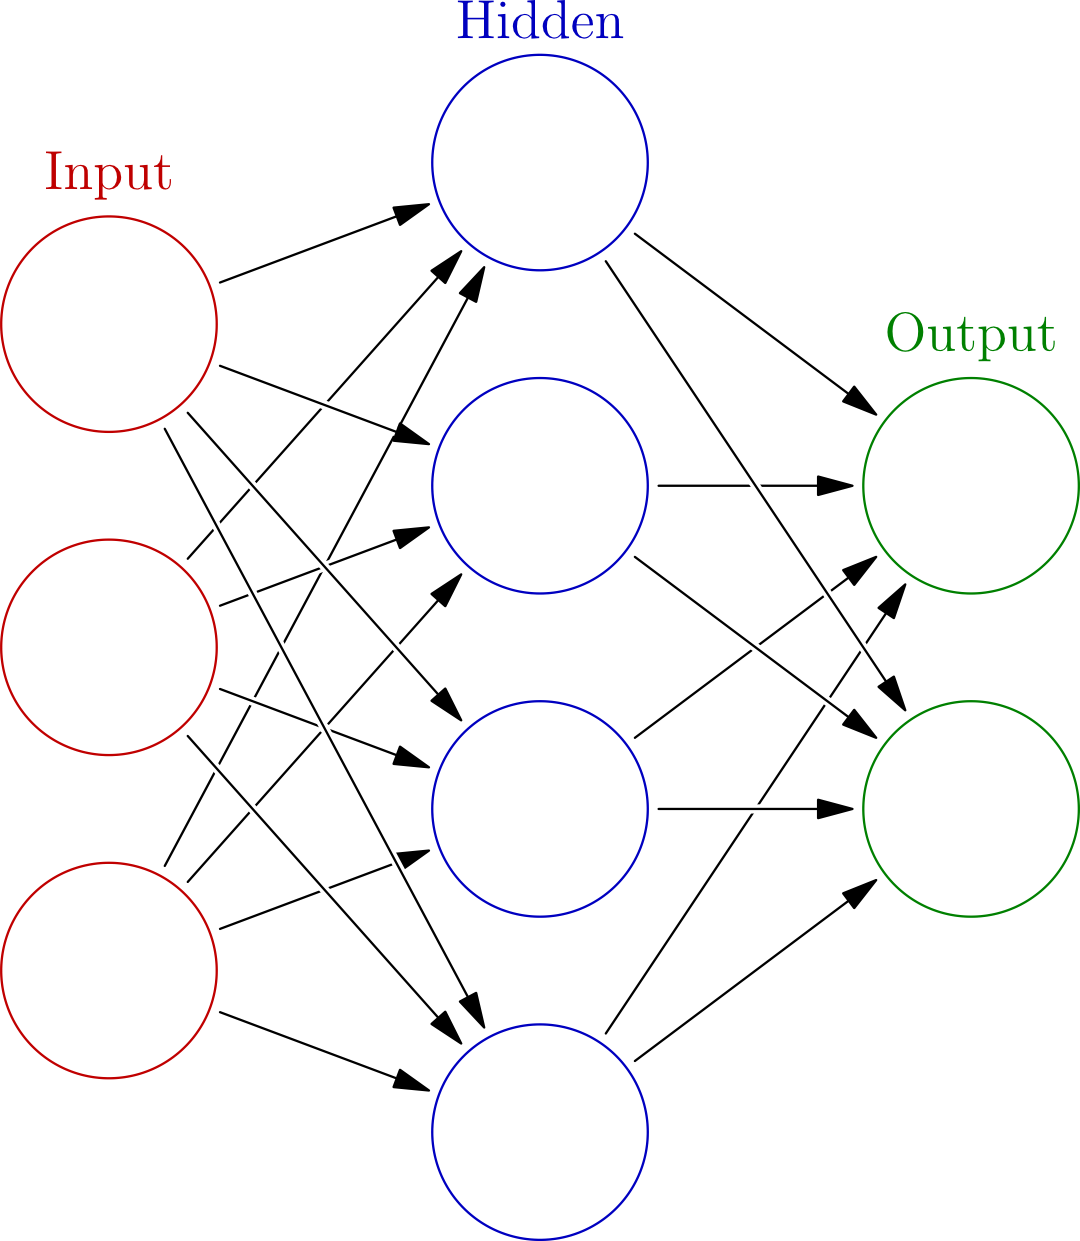
\includegraphics[height=.2\textheight]{../img/colored_neural_network.png}
  \caption{A~simple neural network}
  \label{fig:neural_network}
\end{figure}

\begin{description}
  \item [Convolutional neural network] (CNN) is \todo.
  \item [Deep neural network] is \todo.
\end{description}

\section{Rules of Go}
\emph{Black} and \emph{White} place pieces (\emph{stones}) on the unoccupied intersections (\emph{points}) of a~\emph{board} with a~$19\times19$ grid of~lines.
They take turns, Black moves first.
\begin{description}
  \item [The rule of liberty]
    Every stone remaining on the board must have at least one open point (an~intersection, called a~\emph{liberty}) directly next to it (up, down, left, or right), or must be part of a~connected group that has at least one such liberty next to it.

    Stones or groups of stones which lose their last liberty are removed from the board.

  \item [The ``ko'' rule]
    The stones on the board must never repeat a~previous position of~stones.
    This is to prevent unending cycles.
\end{description}

There are several scoring rules to determine the winner of a~game.
In the match against Lee Sedol, the \emph{area scoring} was used:
a~player's score is the number of player's stones on the board, plus the number of~empty intersections surrounded by that player's stones.

\section{AlphaGo}
\begin{figure}[H]
  \centering
  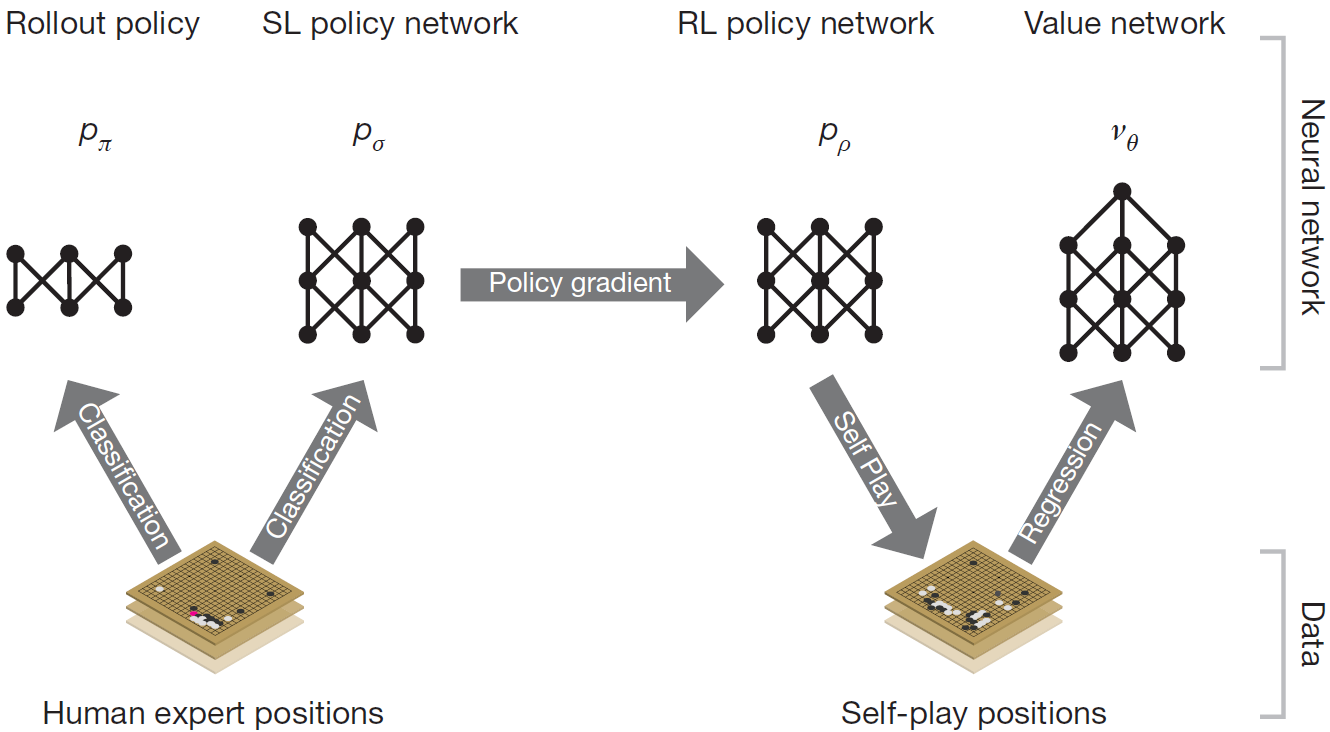
\includegraphics[width=.7\textwidth]{../img/neural_nets_pipeline.png}
  \caption{Training of neural networks: pipeline and architecture}
  \label{fig:neural_nets_pipeline}
\end{figure}

\begin{description}
  \item [Rollout policy] $p_\pi$ is a~CNN rapidly sampling actions during a~\emph{rollout} (a~fast-forward simulation from a~position to the end of~the game).
    It predicts expert human moves faster but less accurately than $p_\sigma$ (see below).
    %The output is a~probability distribution over all moves.

  \item [Policy network] is a~CNN selecting moves.
    It addresses the problem of the game-tree breadth.
    %Again, the output is a~probability distribution over all moves.
    \begin{description}
      \item [SL policy network] $p_\sigma$ is trained by \underline{s}upervised \underline{l}earning to predict expert human moves.
        \item [RL policy network] $p_\rho$ is trained by \underline{r}einforcement \underline{l}earning to win in the~games of~self-play.
    \end{description}

  \item [Value network] $v_\theta$ is a~CNN evaluating board positions to address the problem of the game-tree depth.
    It is trained by regression to predict the outcome in~positions of~the self-play games.
    %The output probability predicts the winner of~games played by the RL policy network against itself.
\end{description}

\begin{theorem}
  The (distributed) AlphaGo program has reached the super-human level of~expertise in~the game of~Go.
\end{theorem}

\begin{proof}
  The proof is left as an exercise to the reader.
  The exercise is to follow the slides.
  :-)
\end{proof}

% Test of Czech: Příliš žluťoučký kůň úpěl příšerné ódy.
% 
% Some text about the paper. 
% quaeram te, domine, invocans te, et invocem te credens in te: praedicatus enim es nobis.
% invocat te, domine, fides mea, quam dedisti mihi, quam inspirasti mihi per humanitatem 
% filii tui, per ministerium praedicatoris tui.
% 
% Second paragraph. Hope you like it.
% 
% \section{More formally}
% 
% \begin{definition}
% Magnus es, domine, et laudabilis valde: magna virtus tua, et sapientiae tuae non est numerus. 
% et laudare te vult homo, aliqua portio creaturae tuae, et homo circumferens mortalitem suam.
% \end{definition}
% 
% \begin{lemma}
% Sed quis te invocat nesciens te? aliud enim pro alio potest invocare nesciens. 
% an potius invocaris, ut sciaris? quomodo autem invocabunt, in quem non crediderunt.
% \end{lemma}
% 
% \begin{theorem}
% The very nice result.
% \end{theorem}
% 
% \begin{proof}
% A sketch of proof if You like. Maybe [1] is used here.
% \end{proof}
% 
% \begin{corollary}
% Some more talking about the article.
% \end{corollary}
% 
% And even more talking about the article. 
% 
% \begin{conjecture}
% Maybe this holds.
% \end{conjecture}
% 
% \begin{exercise}
% Prove that $1+1=3$.
% \end{exercise}
% 
% \section{References}
% 
% [1] F. Havet and M.-L. Yu:
%     $(d,1)$-total labelling of graphs, \textit{Technical Report 4650}, INRIA,
%     2002.
% 
% [2] F. Havet:
%     $(d,1)$-total labelling of graphs, \textit{Workshop Graphs and Algorithms}, Dijon (FRANCE),
% 	2003.

\end{document}
